\documentclass[oneside, 11pt]{article}

\usepackage[T1]{fontenc}
\usepackage[utf8]{inputenc}
\usepackage[english]{babel}

\usepackage{fouriernc}
\usepackage[detect-all, binary-units, separate-uncertainty=true,
            per-mode=symbol, retain-explicit-plus, retain-unity-mantissa=false]{siunitx}

\usepackage{setspace}
\setstretch{1.2}

\setlength{\parskip}{\smallskipamount}
\setlength{\parindent}{0pt}

\usepackage[headheight=14pt]{geometry}
\geometry{marginparwidth=0.5cm, verbose, a4paper, tmargin=3cm, bmargin=3cm,
          lmargin=2cm, rmargin=2cm}

\usepackage{float}

\usepackage[fleqn]{amsmath}
\numberwithin{equation}{section}
\numberwithin{figure}{section}

\usepackage{graphicx}
\graphicspath{{images/}{../../../images/}}

\usepackage{tikz}
\usetikzlibrary{shapes}
\usetikzlibrary{plotmarks}

\newcounter{Exercise}
\setcounter{Exercise}{1}
\usepackage{xcolor}
\definecolor{shadecolor}{gray}{0.9}
\usepackage{framed}
\usepackage{caption}

\usepackage{url}


\usepackage{fancyhdr}
\pagestyle{fancy}
\fancyhf{}
\rhead{\thepage}
\renewcommand{\footrulewidth}{0pt}
\renewcommand{\headrulewidth}{0pt}

\fancypagestyle{firststyle}
{
    \fancyhf{}
    \rhead{\thepage}
    \cfoot{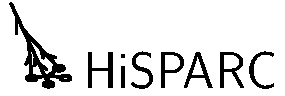
\includegraphics[height=30pt]{HiSPARClogo}}
    \rfoot{
\includegraphics[height=25pt]{CCbysa}}
    \lfoot{
\includegraphics[height=30pt]{NIKHEFlogo}}
    \renewcommand{\footskip}{50pt}
    \renewcommand{\footrulewidth}{0.1pt}
    \renewcommand{\headrulewidth}{0pt}
}

\newcommand{\figref}[1]{Figuur~\ref{#1}}

\newcommand{\hisparc}{\textsmaller{HiSPARC}\xspace}
\newcommand{\kascade}{\textsmaller{KASCADE}\xspace}
\newcommand{\sapphire}{\textsmaller{SAPPHiRE}\xspace}
\newcommand{\jsparc}{\textsmaller{jSparc}\xspace}
\newcommand{\hdf}{\textsmaller{HDF5}\xspace}
\newcommand{\aires}{\textsmaller{AIRES}\xspace}
\newcommand{\csv}{\textsmaller{CSV}\xspace}
\newcommand{\python}{\textsmaller{PYTHON}\xspace}
\newcommand{\corsika}{\textsmaller{CORSIKA}\xspace}
\newcommand{\labview}{\textsmaller{LabVIEW}\xspace}
\newcommand{\daq}{\textsmaller{DAQ}\xspace}
\newcommand{\adc}{\textsmaller{ADC}\xspace}
\newcommand{\hi}{\textsc{h i}\xspace}
\newcommand{\hii}{\textsc{h ii}\xspace}
\newcommand{\mip}{\textsmaller{MIP}\xspace}
\newcommand{\hisparcii}{\textsmaller{HiSPARC II}\xspace}
\newcommand{\hisparciii}{\textsmaller{HiSPARC III}\xspace}

\DeclareSIUnit{\electronvolt}{\ensuremath{\mathrm{e\!\!\:V}}}

\DeclareSIUnit{\unitsigma}{\ensuremath{\sigma}}
\DeclareSIUnit{\mip}{\textsmaller{MIP}}
\DeclareSIUnit{\adc}{\textsmaller{ADC}}

\DeclareSIUnit{\gauss}{G}
\DeclareSIUnit{\parsec}{pc}
\DeclareSIUnit{\year}{yr}



\begin{document}

\title{Deeltjes binnen het standaardmodel}
\author{N.G. Schultheiss}
\date{}

\maketitle
\thispagestyle{firststyle}

\section{Inleiding}

Rond het jaar 1900 was de samenstelling van atomen het onderwerp van
onderzoek. Joseph John Thomson (1856-1940) dacht dat atomen een soort
krentenbollen (eigenlijk plum pudding) waren waar de elektronen als
krenten in zaten. Johannes Wilhelm Geiger \footnote{Johannes Wilhelm
Geiger is ook bekend van de Geiger-Müller-teller, die hij samen met
Walther Müller (1905-1979) in 1928 ontwikkelde.} (1882-1945) en Ernest
Marsden (1889-1970), twee studenten bij Ernest Rutherford (1871-1937),
toonden echter met een experiment in 1909 aan dat atomen grotendeels
leeg zijn. Het blijkt dat als goudfolie (of aluminiumfolie) wordt
bestraald met straling uit Radium, de meeste straling door de folie heen
gaat. Een klein deel van de straling wordt weg- en zelfs teruggekaatst.
Dit resultaat is te verklaren als atomen bestaan uit een kleine kern in
een wolk elektronen.

\begin{figure}[H]
\noindent \begin{centering}
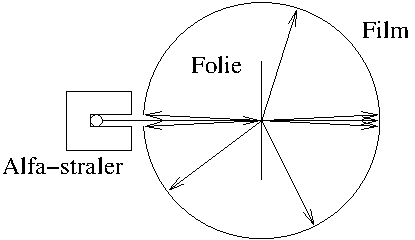
\includegraphics[scale=1]{rutherford}
\par\end{centering}

\caption{Het Rutherford-experiment}


\end{figure}


Een volgend onderwerp voor onderzoek was de samenstelling van de kern.
Rond 1919 komt Rutherford tot de conclusie dat kernen zijn te veranderen
door ze te bestralen met $\alpha$-deeltjes (He-kernen). Het blijkt
dat de positieve lading van de kern verandert. Het atoom heeft na
het bestralen ook andere chemische eigenschappen. Dit is te verklaren
met ``protonen''. In 1932 ontdekte James Chadwick (1891-1974) het
neutron. Hiermee zijn naast elektronen dus ook twee verschillende
kerndeeltjes gevonden. 

Deze elektronen, protonen en neutronen zijn te herkennen aan verschillende
eigenschappen. Zo kunnen we de massa en de elektrische lading van
deze deeltjes bepalen. Sommige elementen, die uit deze deeltjes zijn
samengesteld, zijn radioactief. Deze elementen vervallen, na een bepaalde
tijd (de halfwaardetijd) is de helft over.

In 1922 toonden Otto Stern (1888 - 1969) en Walther Gerlach (1889 -
1979) aan dat zilveratomen als geheel een spin hebben. De zilveratomen
werden door een magnetisch veld op een scherm geschoten. Op het scherm
ontstond geen doorlopende zilverlijn maar twee vlekken met zilveratomen.
Blijkbaar hebben zilveratomen een gequantiseerde magnetische eigenschap,
deze wordt spin \footnote{Omdat spin gequantiseerd is, is er blijkbaar
een soort elementair magneetje.} genoemd. In 1926 toonden Samuel Abraham
Goudsmit (1902 - 1978) en George Eugene Uhlenbeck (1900 - 1988) aan dat
elektronen ook spin hebben.

Ook de configuratie van elektronen rond de kern leidde tot veel onderzoek
door Niels Bohr (1885-1962), Erwin Schrödinger (1887-1961) en vele
anderen. De banen worden berekend met een nieuw soort natuurkunde;
de quantummechanica. Zoals in de module ``de Broglie'' te lezen
is, kent een waterstofatoom een aantal exact gedefinieerde elektronbanen.
De energie van elektronen in de banen is niet continu maar gequantiseerd.
De energieovergangen tussen deze banen zijn daarmee ook vastgelegd.
Er ontstaat een spectrum met absorbtie- of emissielijnen. Omdat elektronen
magnetische deeltjes zijn, kunnen deze banen met een sterk magnetisch
veld gesplitst worden. Soms wijst de spin in de richting van het magnetisch
veld, soms zijn spin en magnetisch veld tegengesteld gericht. Er is
dus een verschil in ``magnetische energie''. Zeeman toonde aan dat
iedere lijn in een spectrum wordt gesplitst als men de lichtbron in
een magnetisch veld zet. 


\section{Versnellers}

Nadat tijdens de tweede wereldoorlog veel onderzoek is gedaan naar
kernwapens, gaat het onderzoek naar de samenstelling van de materie
verder met deeltjesversnellers. Er zijn globaal twee soorten versnellers,
lineaire versnellers en cyclotrons of cirkelvormige versnellers.

In 1945 verzon Luis Walter Alvarez (1911 - 1988) hoe hij uit surplus
materiaal uit de tweede wereldoorlog een lineaire versneller kon bouwen.
Deze versnellers bestonden uit een vacuumbuis waarin een elektrisch
geladen deeltjes worden afgeschoten. In de buis zijn vervolgens ringen
met een wisselende spanning geplaatst. Omdat gelijke ladingen afstoten
en verschillende ladingen aantrekken, kunnen we de deeltjes versnellen
door de spanning om te keren als een deeltje door een ring vliegt.
Eigenlijk wordt er elektrische energie ($E=q*\triangle V$) omgezet in
kinetische of bewegingsenergie ($E=\frac{1}{2}mv^{2}$) van het deeltje.
Deze energie is nu makkelijk te bepalen als we weten hoeveel elementaire
lading het deeltje heeft en hoeveel spanning er tussen twee
opeenvolgende ringen staat. De lading maal de spanning geeft direct de
energie in eV \footnote{De eenheid {[}eV{]} is het product van {[}e{]}
de elementaire lading en {[}V{]} of
$\left[\mathrm{\frac{J}{C}}\right]$.}.

\begin{figure}[h]
\noindent \begin{centering}
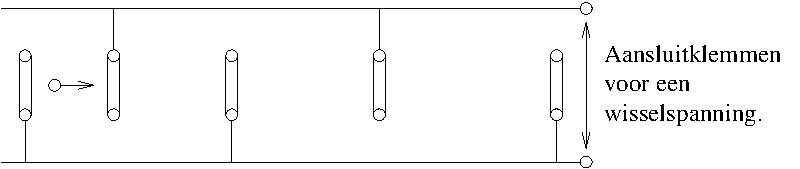
\includegraphics[scale=1]{versneller1}
\par\end{centering}

\caption{Een schematische voorstelling van een lineaire versneller}
\end{figure}


\paragraph*{Opdracht 1:}

\emph{Bereken hoeveel Joule een energiehoeveelheid van }6.6GeV\emph{
is.}


\paragraph*{Opdracht 2:}

\emph{Bereken de snelheid van een proton als deze door vijf opeenvolgende
ringen vliegt. Neem aan dat de snelheid bij de eerste ring te verwaarlozen
is en het spanningsverschil tussen de ringen 1kV is.}


\paragraph*{Opdracht 3:}

\emph{Leg uit waarom de afstand tussen de ringen steeds groter wordt.}

Lineaire versnellers kunnen deeltjes niet meer dan een beperkte hoeveelheid
energie geven omdat er een beperkt aantal ringen zijn. In een cyclotron
wordt deze beperking opgeheven omdat de deeltjes in een cirkel bewegen.
Om de elektrisch geladen deeltjes in een cirkelbaan te laten bewegen
is een magnetisch veld nodig.

\begin{figure}[h]
\noindent \begin{centering}
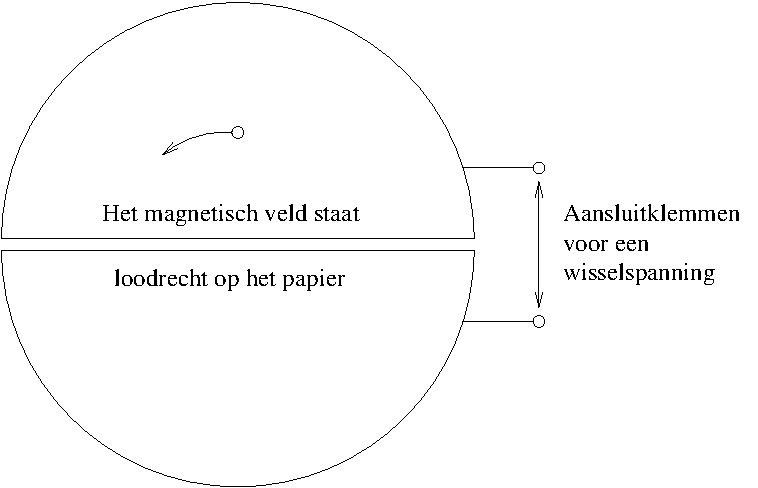
\includegraphics[scale=0.75]{versneller2}
\par\end{centering}

\caption{Een schematische voorstelling van een cyclotron}
\end{figure}


Iedere keer als het deeltje in figuur 2.2 een halve cirkel aflegt,
krijgt het deeltje een extra zetje. Omdat het deeltje steeds sneller
gaat, zal de straal van de baan steeds groter worden. Volgens Einstein
kunnen deeltjes echter niet sneller gaan dan de lichtsnelheid. Volgens
de formule $E=mc^{2}$ wordt de energie dan omgezet in extra massa.


\paragraph*{Opdracht 4:}

\emph{Wat kun je over de omlooptijd van het deeltje in de cyclotron
zeggen als de wisselspanning een constante frequentie heeft? Hoe kan
een deeltje dan toch een grotere snelheid krijgen?}

Ernest Orlando Lawrence (1901 \textendash{} 1958) begon in 1929 met
de ontwikkeling van cyclotrons. In 1954 resulteerde dit in het Bevatron
in het Lawrence Berkeley National Laboratory. Met deze versneller
konden protonen worden versneld tot een energie van 6,6GeV. De protonen
hebben dan volgens Einstein een massa van $6,6\frac{\mathrm{GeV}}{c^{2}}$. 


\paragraph*{Opdracht 5:}

\emph{Bereken hoeveel maal de protonen zwaarder worden als ze een
energie van }6,6GeV\emph{ krijgen.}

Zoals we weten, is een 1GeV het zelfde als $10^{9}$eV of 1 miljard
eV. Helaas wordt ``een miljard'' in het engels vertaald als ``one
billion''. Als we een ``billion electronVolt cyclotron'' hebben,
is dit dus af te korten tot een Bevatron. Met deze versneller konden
voor het eerst antiprotonen worden gemaakt door protonen te laten
botsen op stilstaande atomen. 

We kennen nu dus al elektronen en anti-elektronen en protonen en
anti-protonen. Het is dus ook mogelijk om een anti-waterstof atoom te
maken \footnote{In 1996 kon men in CERN antiprotonen opslaan in LEAR, de
Low Energy Antiproton Ring. In principe was het maken van antiwaterstof
toen mogelijk.}. 

Na de ontdekking van het anti-proton werd er in 1959 een nieuw deeltje
gevonden: het pion. In eerste instantie vroeg men zich af of het pion
als een soort lijm voor de protonen en neutronen in de kern werkte.
Het heelal werd wel veel ingewikkelder. Zou er een anti-pion zijn?
Zijn er nog meer deeltjes mogelijk? Om dit te onderzoeken zijn grotere
versnellers nodig. Met een grotere versneller kan men meer energie
in een deeltje stoppen. In de module ``De Broglie'' is te lezen
dat meer energie een kleinere golflengte voor het deeltje geeft. We
kunnen dus kleinere deeltjes vinden.

De bundel protonen in het Bevatron had een doorsnede of apertuur van
ongeveer $\frac{1}{3}\mathrm{m}^{2}$. Om een dergelijke grote bundel
rond te laten gaan, heb je een grote magneet nodig. Met een smallere
bundel hebben we minder magneten nodig en kunnen we deeltjes met meer
energie maken. Na de Bevatron kwam de Tevatron die deeltjes een energie
van een teraelektronVolt of $10^{12}$eV kon geven. Op dit moment
zijn er twee onderzoekscentra die de grootste versneller willen bouwen:
CERN in Europa (>2TeV) en Fermilab (2TeV sinds de 80er jaren) in Amerika.
Men hoopt met de LHC (Large Hadron Collider) in Cern deeltjes een
energie te geven van 7TeV. In de LHC lopen twee bundels tegengesteld
met beide op de botsingsplaatsen een diameter van $16\mu\mathrm{m}$.
Omdat er twee bundels botsen, komt er maximaal (botsingscentraal)
14TeV vrij.


\paragraph*{Opdracht 6:}

\emph{Protonen maken in de LHC rondjes van 27}km\emph{ en gaat daarbij
vier keer door een oppervlak met een diameter van $16\mu\mathrm{m}$.
De maan is ongeveer 1lichtseconde van ons weg. Bereken hoe groot een
doel op de maan in verhouding zou zijn als we ons voorstellen dat
de protonen de baan van de maan volgen. }


\section{Quarks}

Uit botsingsproeven met versnellers blijkt dat protonen en neutronen
ook weer uit deeltjes bestaan. Deze worden ``quarks'' genoemd. Zowel
protonen als neutronen bevatten drie quarks.

We kunnen elementaire deeltjes op de volgende manier opdelen:

\noindent \begin{center}
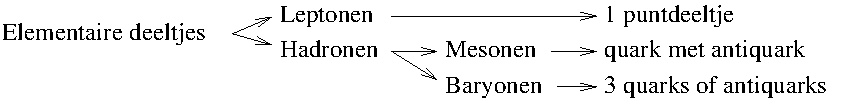
\includegraphics[scale=0.75]{deeltjes}
\par\end{center}

Leptonen zijn deeltjes zoals elektronen, positronen of neutrino's.
Omdat protonen en neutronen uit drie quarks bestaan, moeten dit wel
baryonen zijn. Op mesonen komen we nog terug in de module ``Krachten
binnen het standaardmodel''. 

Het proton bestaat uit 2 ``up'' quarks en 1 ``down'' quark. Het
neutron bestaat uit 2 ``down'' quarks en 1 ''up'' quark. Om een
antideeltje te maken hebben we ook ``anti-up'' quarks en ``anti-down''
quarks nodig. Deze quarks en antiquarks werden met de eerste generatie
versnellers gevonden en worden dan ook eerste generatie quarks genoemd.

Met grotere versnellers kunnen we ook quarks van de tweede en derde
generatie aantonen. Op dit moment kennen we de volgende quarks:

\noindent \begin{center}
\begin{tabular}{|c|c|c|c|c|}
\hline 
Generatie & Spin & Naam & Symbool & Q {[}e{]}\tabularnewline
\hline 
\hline 
1 & 1/2 & up & u & 2/3\tabularnewline
\hline 
1 & -1/2 & down & d & -1/3\tabularnewline
\hline 
2 & -1/2 & strange & s & -1/3\tabularnewline
\hline 
2 & 1/2 & charm & c & 2/3\tabularnewline
\hline 
3 & -1/2 & bottom & b & -1/3\tabularnewline
\hline 
3 & 1/2 & top & t & 2/3\tabularnewline
\hline 
\end{tabular}
\par\end{center}

Dit model is door Murray Gell-Mann (1929) uit de groepentheorie ontwikkelt
en staat bekent als SU(3) of het achtvoudig pad. Het valt op dat quarks
een lading hebben, deze is +$\frac{2}{3}$e en -$\frac{1}{3}$e voor
de quarks en -$\frac{2}{3}$e en +$\frac{1}{3}$e voor de antiquarks.
In de samengestelde deeltjes vinden we alleen ladingen van -2e, -1e,
0e, 1e of 2e. Blijkbaar geeft dit dus een regel voor het samenvoegen
van quarks.


\section{Fermionen en bosonen}

Quarks kunnen op verschillende manieren worden samengevoegd. Het blijkt
dat de spin een belangrijke eigenschap van de uit quarks samengestelde
deeltjes is. De deeltjes zijn nu ook weer in twee groepen te splitsen:
Fermionen en Bosonen.

Fermionen zijn naar Enrico Fermi (1901 \textendash{} 1954) genoemd.
Fermionen zijn deeltjes met een halftallige spin, zoals ....., -3/2,
-1/2, 1/2, 3/2, ..... . Ieder fermion moet in een unieke toestand
zitten. Dit is bijvoorbeeld te zien in het He-4 atoom. De 2 protonen
en de 2 neutronen zitten in de kern. Protonen, neutronen en elektronen
maken deel uit van de fermionen. Rond de kern draaien ook 2 elektronen.
In het geval dat de energie op zijn laagst is, zitten beide elektronen
in de schil die het dichtst bij de kern is. Op het eerste gezicht
lijken de elektronen dus beide in dezelfde toestand te zijn. Het ene
electron heeft echter een spin van 1/2 en het andere een spin van
-1/2. De toestand is dus op de spin na hetzelfde. Omdat de spin verschilt,
verschilt de toestand waarin de elektronen zich bevinden ook. Hieruit
volgt dat er niet meer dan twee elektronen in een orbitaal (baan)
zitten.

Het feit dat twee gelijke toestanden uitgesloten zijn, heet ook wel
het Pauli-principe. Dit principe is in 1925 geformuleerd door Wolfgang
Ernst Pauli (1900 \textendash{} 1958)

Bosonen zijn naar Satyendra Nath Bose (1894 \textendash{} 1974) genoemd.
Bosonen hebben een heeltallige spin, zoals ....., -2, -1, 0, 1, 2,
..... . Het He-4 atoom is als geheel te beschouwen als een boson.
Er zijn 6 deeltjes met ieder een spin van 1/2 of -1/2. Als we alle
mogelijke combinaties voor de spin bekijken, komt de som altijd op
een geheel getal uit. 

Als He-4 wordt afgekoeld, ontstaat er een bijzondere toestand. Dit
Bose-Einstein condensaat gedraagt zich niet meer als een verzameling
atomen maar als een geheel.

Omdat er geen Pauli-uitsluiting is, stroomt het He naar de laagste
energie toestand. Als het in een potje zit, stroomt het er vanzelf
uit.


\paragraph*{Opdracht 7:}

\emph{Zoek een filmpje over supervloeibaar Helium. Ik heb en filmpje
gevonden op:}

\url{https://youtu.be/TBi908sct_U} / Superfluid Helium (with Subtitles)


\section{Leptonen}

Leptonen zijn fermionen waarvan men tot op heden aanneemt dat deze
niet gedeeld kunnen worden. Leptonen worden als puntdeeltjes beschouwd.
Het bekendste lepton is het elektron. In de module ``De zon'' hebben
we gezien dat een elektron ook een antideeltje heeft: het positron.
Deze deeltjes hebben ook zwaardere broertjes of zusjes, het muon en
het tauon. Daarnaast zijn er ook nog neutrino's met ook zwaardere
broertjes of zusjes. Volgens Einstein betekent een zwaarder deeltje
dat het meer energie bevat. Omdat deze energie er uit kan, vervallen
deze deeltjes. 

\noindent \begin{center}
\begin{tabular}{|>{\centering}p{3cm}|c|c|c|c|c|c|c|>{\centering}p{3cm}|}
\hline 
\multicolumn{9}{|c|}{Eigenschappen van leptonen}\tabularnewline
\hline 
\hline 
Naam deeltje / antideeltje & Symbool & Q {[}e{]} & S & $\mathrm{L}_{e}$ & $\mathrm{L}_{\mu}$ & $\mathrm{L}_{\tau}$ & Massa {[}$\mathrm{\frac{MeV}{c^{2}}}${]} & Halfwaarde {[}s{]}\tabularnewline
\hline 
Elektron / Positron & $e^{-}/e^{+}$ & \textminus{}1/+1 & 1\textfractionsolidus{}2 & +1/\textminus{}1 & 0 & 0 & 0.510998910 & Stabiel\tabularnewline
\hline 
Muon / Antimuon & $\mu^{-}/\mu^{+}$ & \textminus{}1/+1 & 1\textfractionsolidus{}2 & 0 & +1/\textminus{}1 & 0 & 105.6583668 & $2.197019*10^{-6}$\tabularnewline
\hline 
Tauon / Antitauon & $\tau^{-}/\tau^{+}$ & \textminus{}1/+1 & 1\textfractionsolidus{}2 & 0 & 0 & +1/\textminus{}1 & 1,776.84 & $2.906*10^{-13}$\tabularnewline
\hline 
Elektron neutrino / Elektron antineutrino & $\nu_{e}/\overline{\nu_{e}}$ & 0 & 1\textfractionsolidus{}2 & +1/\textminus{}1 & 0 & 0 & < 0.0000022 & \tabularnewline
\hline 
Muon neutrino / Muon antineutrino & $\nu_{\mu}/\overline{\nu_{\mu}}$ & 0 & 1\textfractionsolidus{}2 & 0 & +1/\textminus{}1 & 0 & < 0.17 & \tabularnewline
\hline 
Tauon neutrino / Tauon antineutrino & $\nu_{\tau}/\overline{\nu_{\tau}}$ & 0 & 1\textfractionsolidus{}2 & 0 & 0 & +1/\textminus{}1 & < 15.5 & \tabularnewline
\hline 
\end{tabular}
\par\end{center}


\section{Baryonen}

Baryonen zijn samengestelde deeltjes waarin 3 quarks zitten. Bekende
baryonen zijn het proton en het neutron. Omdat quarks een spin van
1/2 of -1/2 hebben \footnote{Volgens Zeeman kent de spin twee gequantiseerde toestanden. De spin
is dus altijd gelijkgericht of tegengesteld gericht.}, moeten baryonen ook fermionen zijn. Eén van de quarks kan een tegengestelde
spin aan de andere twee quarks hebben. Er onstaan baryonen met spin
-1/2 of 1/2. Deze deeltjes bevatten up-quarks (\emph{u}) of down-quarks
(\emph{d}). Toen men met versnellers ging meten aan deze deeltjes
ontdekte men vreemde nieuwe deeltjes. Deze deeltjes hebben een relatief
grote halfwaardetijd van $10^{-10}\mathrm{s}$. Om deze deeltjes te
kunnen maken, is er een nieuw quark nodig: het strange-quark (\emph{s}).
Uiteraard kan de spin van drie quarks ook evenwijdig zijn, er ontstaat
dan een deeltje met spin -3/2 of 3/2.

Verder viel het Werner Heisenberg in 1932 (ver voor de ontdekking
van quarks) op dat neutronen en protonen op de lading na vrijwel identiek
waren. Hij beschouwde het neutron daarom als een andere toestand van
het proton. Om dit verschil aan te geven introduceerde hij een nieuwe
eigenschap van nucleonen. Deze eigenschap werd in 1937 door Eugene
Wigner aangeduid met ``isospin'' of $\mathrm{I}_{3}$. In de figuren
6.1 en 6.2 is deze eigenschap langs de horizontale as uitgezet. Langs
de verticale as staat de ``strangeness'' van het deeltje uitgezet.
Zoals te zien is, is deze voor protonen en neutronen 0 omdat deze
geen s-quarks bevatten.

\begin{figure}[h]
\noindent \begin{centering}
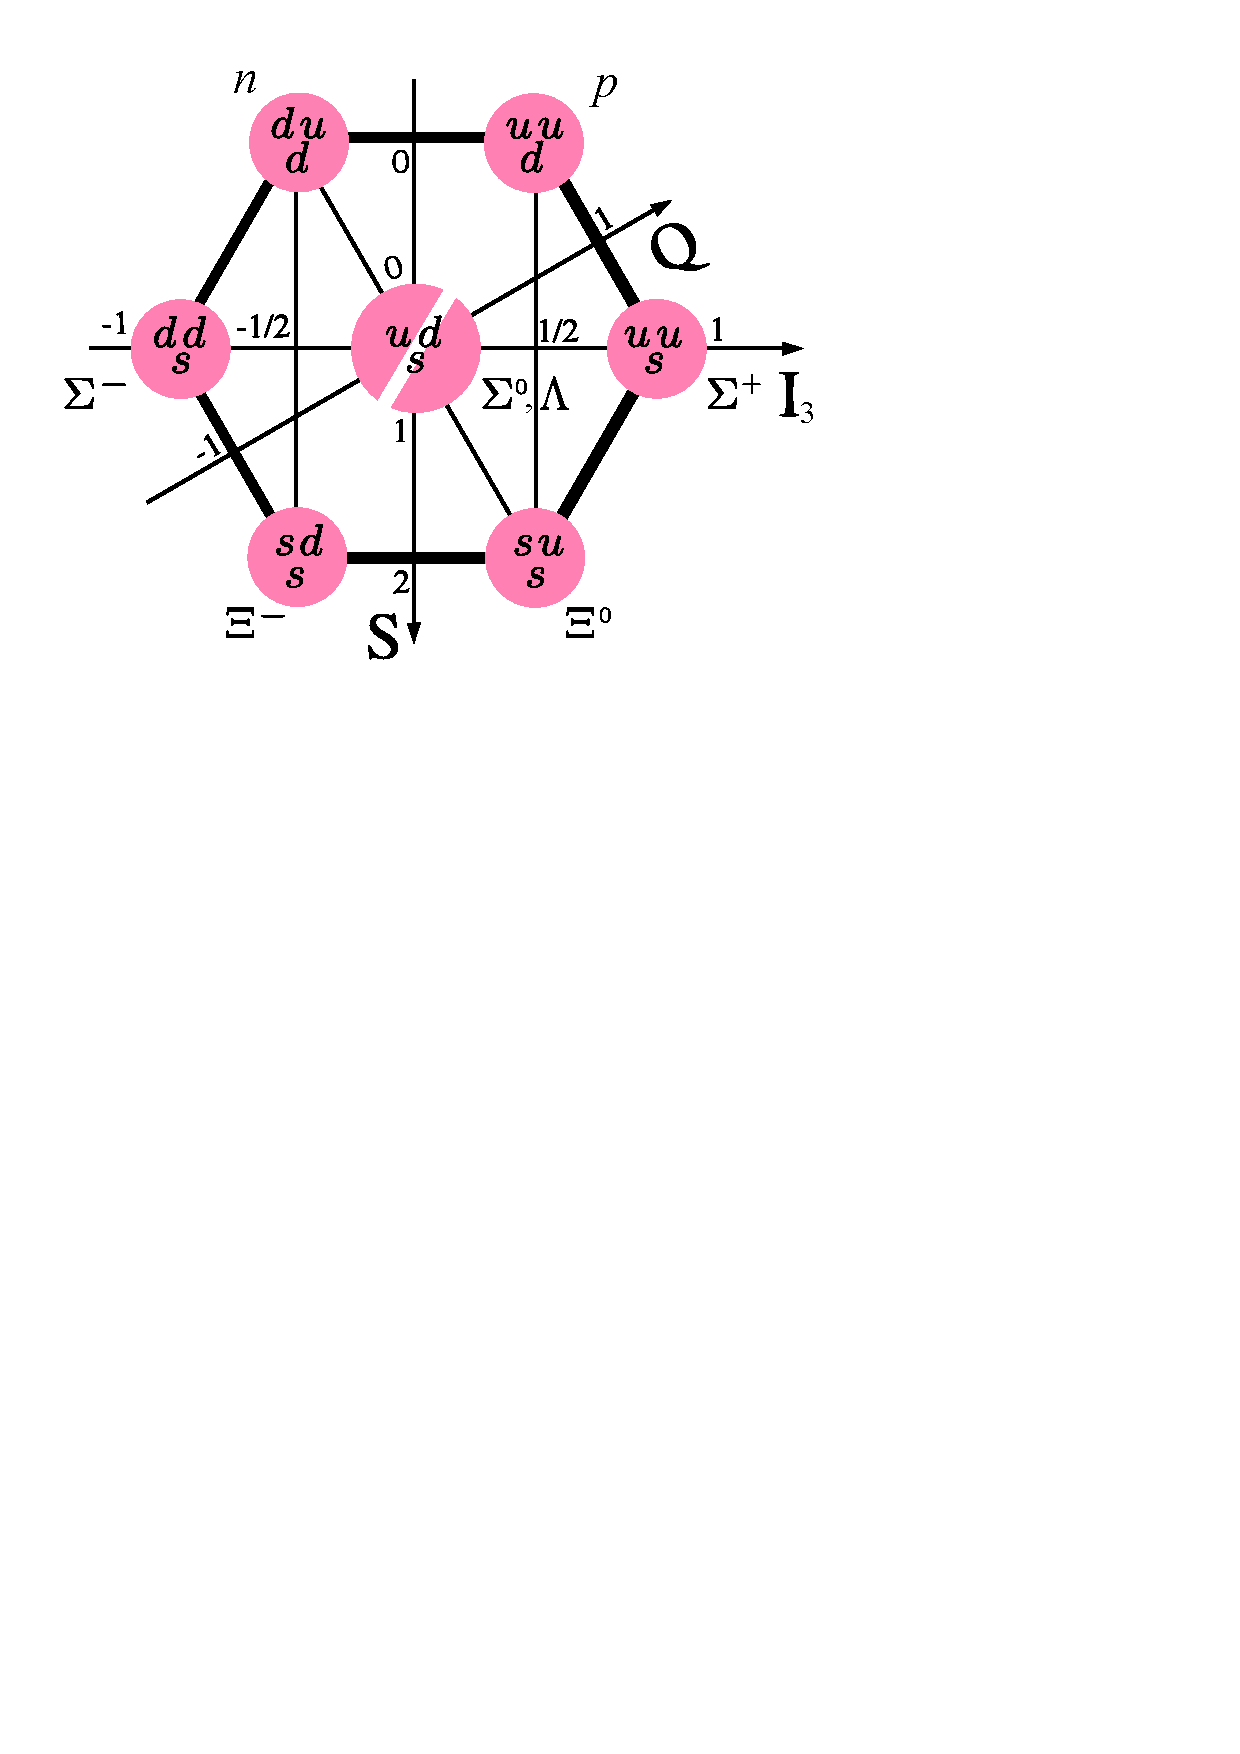
\includegraphics[scale=0.4]{Baryon_octet_small}
\par\end{centering}

\caption{Baryonen met spin -1/2 of spin 1/2}
\end{figure}


Omdat quarks fermionen zijn, kunnen ze natuurlijk alleen in een unieke
quantumtoestand voorkomen. Als er meerdere deeltjes mogelijk zijn,
moeten ze ieder een eigen quantumtoestand hebben en is hier een grootheid
voor te vinden. In de figuren 6.1 en 6.2 (op Wikipedia te vinden),
zijn dit de isospin $\mathrm{I}_{3}$, strangeness S en lading Q.
Het lijkt erop dat de lading het gevolg is van de isospin en de strangeness.
Het verschil tussen figuur 6.1 en 6.2 zit in de spin van het baryon.

Verder valt op dat men een neutron kan veranderen in een $\Delta^{0}$
door de totale spin van het baryon te veranderen (het quark met een
tegengestelde spin bij het neutron krijgt een gelijke spin). Een $\Delta^{0}$
is dus te beschouwen als een aangeslagen neutron. 

We kunnen nu overigens ook verklaren dat er alleen baryonen met ddd-,
uuu-, of sss-quark combinaties zijn als de spin $\frac{3}{2}$ of
$-\frac{3}{2}$ is. De combinatie van de spin is dan uniek. Als de
spin met drie gelijke quarks $\frac{1}{2}$ of $-\frac{1}{2}$ zou
zijn, kunnen er meerdere mogelijkheden zijn om dit met de spin van
de drie quarks te maken. Dit mag niet volgens het Pauli-principe.

\begin{figure}[H]
\noindent \begin{centering}
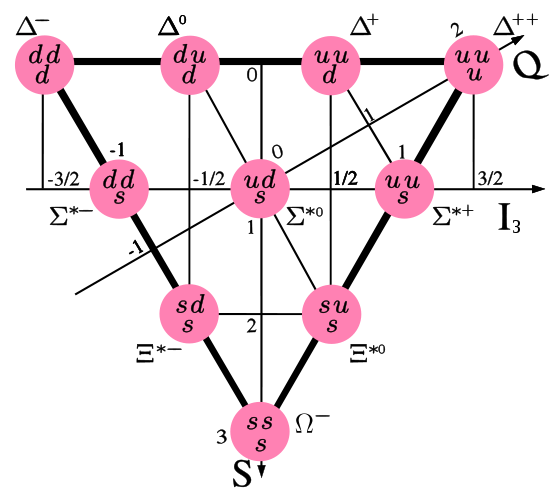
\includegraphics[scale=0.3]{Baryon_decuplet_small}
\par\end{centering}

\caption{Baryonen met spin -3/2 of 3/2}
\end{figure}

\end{document}
